
\section{Performance of the Isolation Requirement}
\label{app:trkvetoperf}

The last requirement used in the analysis is an isolated track
veto. This selection criteria rejects events containing a track of $\pt>10~\GeV$
with relative track isolation $\sum \pt/\pt(trk)$ in a cone of size $R=0.3<0.1$. It may be noted that only tracks consistent with the
vertex with highest $\sum \pt^2$ are considered in order to
reduce the impact of spurious tracks, for example from pileup interactions. This requirement has very good
performance. Figure~\ref{fig:isolvetoroc} shows the
efficiency for rejecting dilepton events compared to the efficiency
for selecting single lepton events for various cone sizes and cut
values. The chosen working point provides a signal efficiency of
$\epsilon(sig) =92\%$ for a background rejection of $\epsilon(bkg)
=53\%$ in MC. With "signal" ("background") we are referring to \ttlj\ (\ttll\ ).

\begin{figure}[hbt]
  \begin{center}
	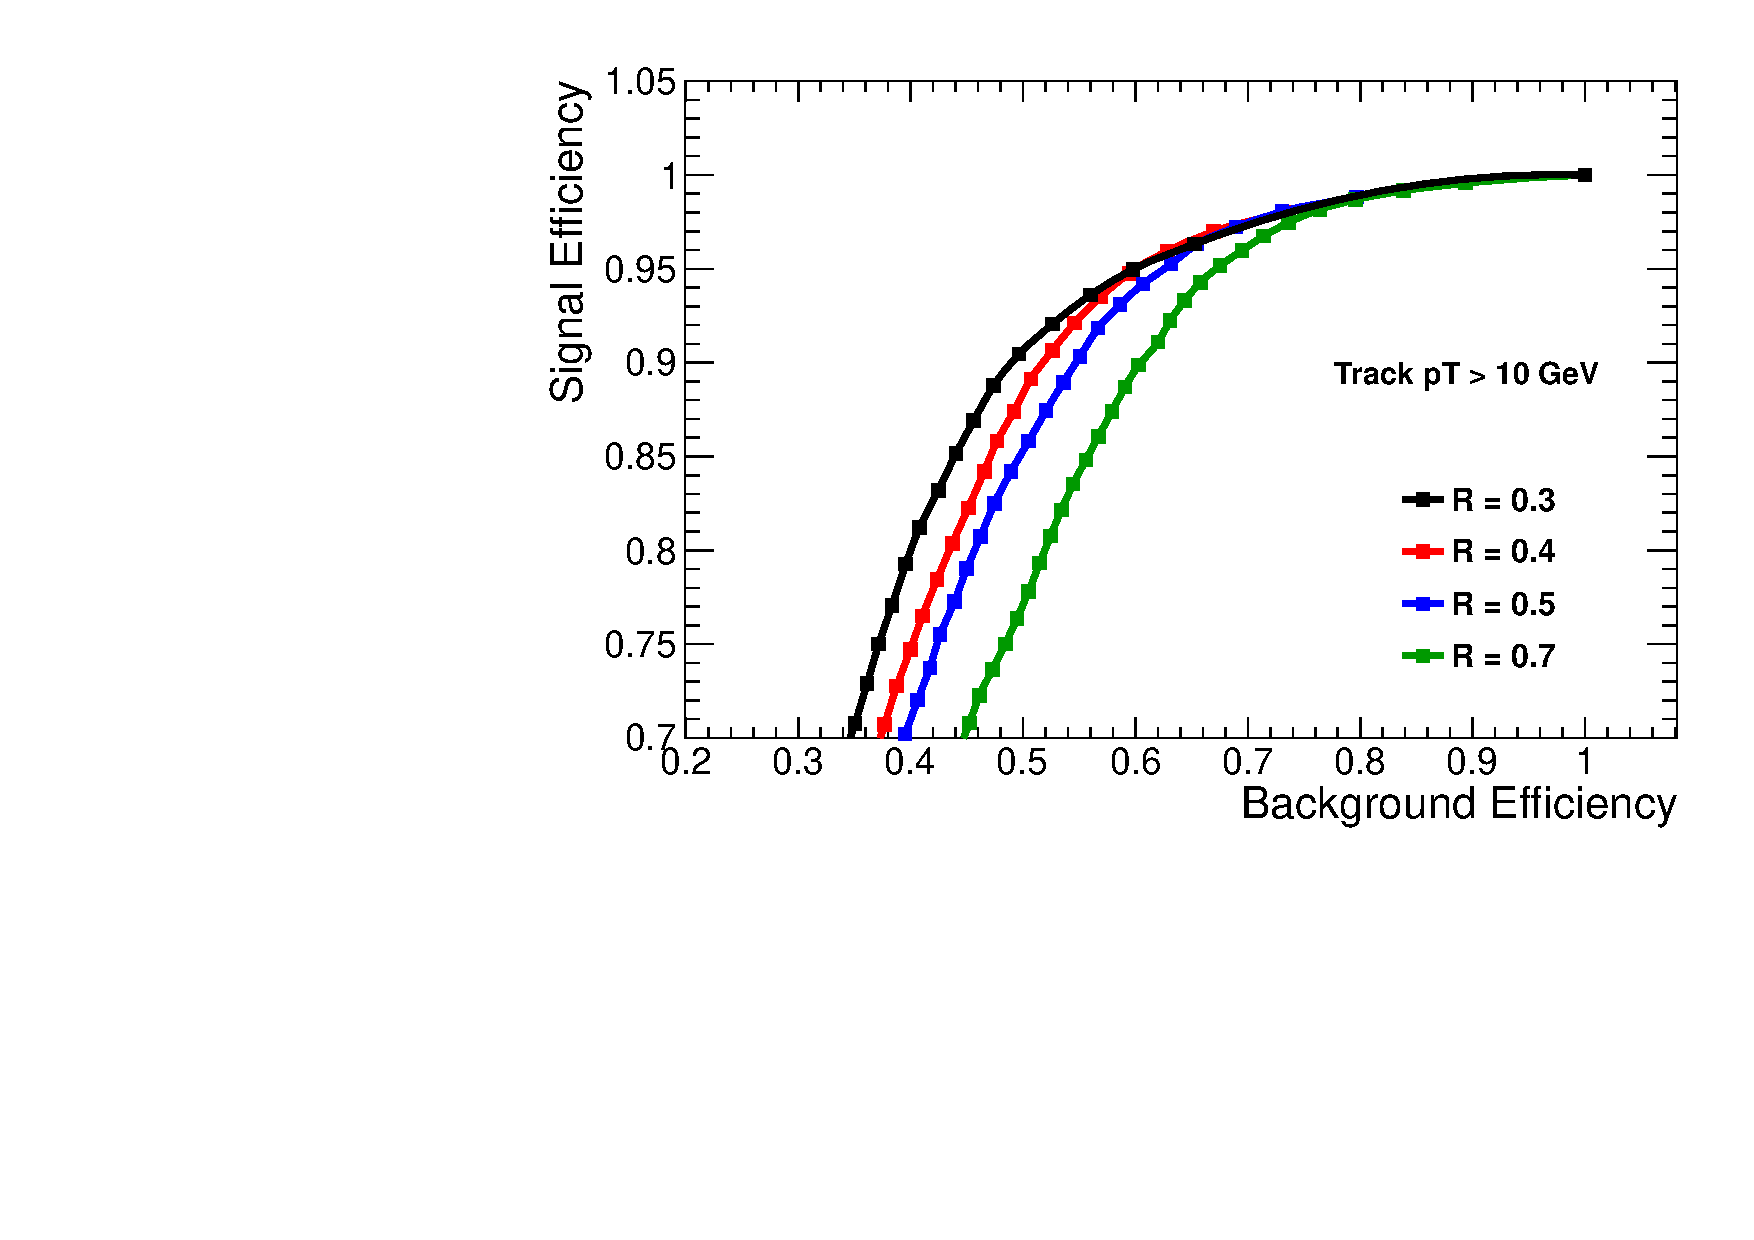
\includegraphics[width=0.7\linewidth]{plots/roc_ttdl_trkiso_pt10.pdf}
	\caption{
	  \label{fig:isolvetoroc}%\protect 
          Comparison of the performance in terms of signal (single lepton events) efficiency
         and background (dilepton events) rejection for various cone
         sizes and cut values. The current isolation requirement uses
         a cone of size $\Delta R = 0.3$ and a cut value of 0.1,
         corresponding to $\epsilon(sig) =92\%$ for $\epsilon(bkg)=53\%$.
       ADD ARROW OR LINE TO INDICATE WORKING POINT.}  
      \end{center}
\end{figure}

It should be emphasized that the isolated track veto has a different impact on the samples with a single
lepton (mainly \ttlj\ and \wjets) and that with two leptons (mainly \ttll).
For the dilepton background, the veto rejects events which have a
genuine second lepton. Thus the performance may be understood
as an efficiency $\epsilon_{iso\ trk}$ to identify the isolated track. In the
case of the single lepton background, the veto rejects events
which do not have a genuine second lepton, but rather which contain 
a ``fake'' isolated track. The isolated track veto thus effectively scales the
single lepton sample by (1-$\epsilon_{fake}$), where $\epsilon_{fake}$ is the probability to 
identify an isolated track with \pt $> 10$~\GeV in events which contain no genuine second
lepton. It is thus necessary to study the isolated track efficiency
$\epsilon(trk)$ and $\epsilon_{fake}$ in order to fully
characterize the veto performance. 

The veto efficiency for dilepton events is calculated using 
the tag and probe method in \Z\ events. A good lepton
satisfying the full ID and isolation criteria and matched to a
trigger object serves as the tag. The probe is defined as a track with
$\pt>10~\GeV$ that has opposite charge to the tag and has an invariant
mass with the probe consistent with the \Z\ mass. 

{\bf Fix me: fkw does not understand why you refer to \pt $>$ 10~\GeV here, given that in the very next paragraph you state that
this is measured via the absolute track isolation, implying, but not explicitly stating, that a much higher \pt\ threshold is used to get a clean Z signal. ???}

The variable used to study the performance of the veto is the absolute track isolation,
since it removes the dependence of the isolation variable on the \pt\ of the
object under consideration. This is particularly useful because the
underlying \pt\ distribution is different for second leptons in
\ttll\ events compared to \Z\ events, particularly due to the presence of $\tau$s
that have softer decay products. As shown in Figure~\ref{fig:absiso}, the absolute
isolation is consistent between $\Z+4$ jet events and \ttll\ events,
including leptons from \W\ and $\tau$ decays. This supports the notion
that the isolation, defined as the energy surrounding the object under
consideration, depends only on the environment of the object and not
on the object itself. The isolation is thus sensitive to the ambient
pileup and jet activity in the event, which is uncorrelated with
the lepton \pt. It is thus justified to use tag and probe in
$\Z+4$ jet events, where the jet activity is similar to \ttll\
events in our \njets\ $>$ 4 signal region, in order to estimate the performance of the isolation 
requirement for the various leptonic categories of \ttll\ events. 

\begin{figure}[hbt]
  \begin{center}
	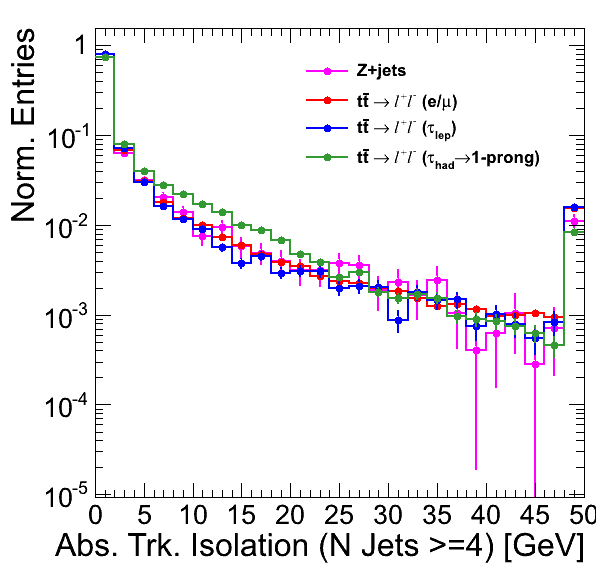
\includegraphics[width=0.5\linewidth]{plots/pfabsiso_njets4_log.png}%
	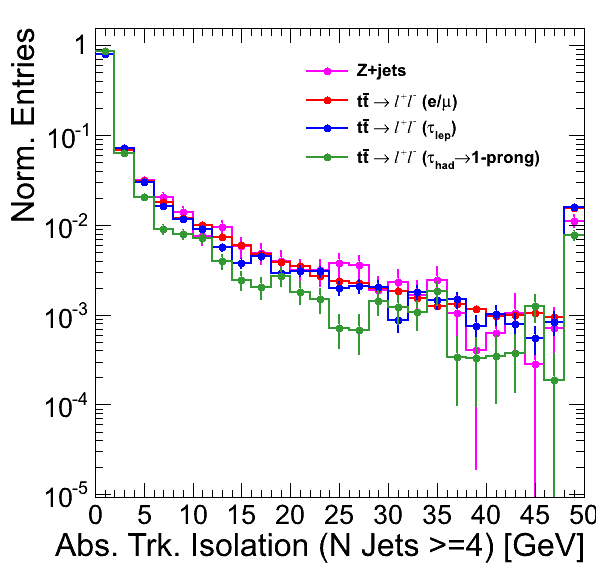
\includegraphics[width=0.5\linewidth]{plots/pfabsiso_njets4_clean_log.png}
	\caption{
	  \label{fig:absiso}%\protect 
          Comparison of absolute track isolation for track probes in
          $\Z+4$ jet and \ttll\ events for different lepton types. The
          isolation variables agree across samples, except for single
          prong $\tau$s, that tend to be slightly less isolated
          (left). The agreement across isolation distributions is
          recovered after removing single prong $\tau$ events produced 
          in association with $\pi^0$s from the sample (right).}  
      \end{center}
\end{figure}

%It may be noted that tracks from single prong $\tau$ decays are
%slightly less isolated compared to electrons and muons. The reason is that single
%prong $\tau$s can have $\pi^0$ associated with the single charged
%track. These decay into $\gamma$s that in turn convert $\gamma\to e^+e^-$ and spoil the
%isolation. As also shown in Figure~\ref{fig:absiso},
%the isolation distribution for charged tracks from $\tau$ decays that
%are not produced in association with $\pi^0$s are consistent with that
%from $\E$s and $\M$s. Since events from single prong
%$\tau$ decays produced in association with $\pi^0$s comprise a small
%fraction of the total sample, the isolation measured for leptons is used
%for all single prong $\tau$ events. A systematic uncertainty is
%assigned to account for the difference in the underlying
%isolation distribution for this sample.
